\documentclass[12pt, a4paper]{article}
\usepackage[UTF8]{ctex}
\usepackage{amsmath}
\usepackage{amssymb}
\usepackage{amsthm}
\usepackage{geometry}
\usepackage{enumitem}
\usepackage{indentfirst}
\usepackage{caption}
\usepackage{fancyhdr}
\usepackage{booktabs}
\usepackage{titlesec}
\usepackage{draftwatermark}
\usepackage{graphicx} % 导入图像的宏包、单图





% 页面布局设置
\geometry{top=2.54cm, bottom=2.54cm, left=3.18cm, right=3.18cm}

% 行距设置
\linespread{1.5}

%设置水印
\SetWatermarkText{B站：布加拉提}
\SetWatermarkScale{0.4}
% 段落设置
\setlength{\parindent}{2em}
\setlength{\parskip}{0.5em}

% 节标题格式设置
\titleformat{\section}{\normalfont\Large\bfseries}{第\chinese{section}章、}{1em}{}
\titlespacing{\section}{0pt}{2.5ex plus 1ex minus .2ex}{1.3ex plus .2ex}

% 定理环境设置
\newtheoremstyle{solution}
{}
{}
{}
{}
{\bfseries}
{、}
{1em}
{}
\theoremstyle{solution}
\newtheorem{sol}{解}

% 页眉页脚设置
\pagestyle{fancy}
\fancyhf{}
\fancyhead[C]{b站布加拉提整理（回忆版）b站甘茶w独家讲解}
\fancyfoot[C]{\thepage}

\rfoot{整理人：八方\\资源提供：考研乔瑟夫}
\lhead{
\includegraphics[width=0.06\linewidth]{p1.png}}
\rhead{
\includegraphics[width=0.06\linewidth]{p2.png}}
\renewcommand{\headrulewidth}{0.4pt}
\renewcommand{\footrulewidth}{0.4pt}

\begin{document}

\begin{center}
\Large\textbf{2007哈工大硕士考试试题：805物理光学}
\end{center}




\section*{一、填空与选择（28分）}
\begin{enumerate}
    \item 两光波发生干涉的必要条件为\_\_\_\_\_,\_\_\_\_\_,\_\_\_\_\_补充条件为\_\_\_\_\_。
    \item 获得相干光的方法有\_\_\_\_\_,\_\_\_\_\_两种。
    \item 单色光波(自然光)从折射率为$n_1$的透明介质1空间射入折射率为$n_2$的透明介质2空间，在两介质的分界面上发生\_\_\_\_\_和\_\_\_\_\_现象；反射角$\theta_1$,透射角$\theta_2$和入射角$\theta_3$的关系为\_\_\_\_\_和\_\_\_\_\_;设$\lambda_1$和$\lambda_2$分别为光波在介质1，介质2中的波长，则$\lambda_1$和$\lambda_2$的关系为\_\_\_\_\_；反射光波发生相位跃变的条件是\_\_\_\_\_，发生全反射
的条件是\_\_\_\_\_，反射光波为线偏振光的条件是\_\_\_\_\_。
    \item 法布里-珀干涉仪利用平板的\_\_\_\_\_工作原理，其光谱分辨本领为\_\_\_\_\_。
    \item 使自然光相继通过三个偏振片，第一个与第三个偏振片的透光轴（从偏振光透出的偏振光的振动方向）正交，第二个偏振片的透光轴与第一个偏振片的透光轴成$30^\circ$角，若入射自然光的强度为$I_0$，则最后透出的光强为\_\_\_\_\_。
    \item 某激光的频宽为$6.0\times10^{4}Hz$，其波列长度为\_\_\_\_\_.\\(A) $5.55\times10^{3}m$ \quad (B) $1.8\times10^{3}m$ \quad (C) $5.55\times10^{4}m$ \quad (D) $5.0\times10^{3}m$
    \item （重复）在真空中波长为$\lambda$的单色光，在折射率为$n$的透明介质中从A沿路径传播到B，若A、B两点的相位差为$5\pi$，则此路径AB的光程差为\_\_\_\_\_.\\(A) $2.5\lambda$ \qquad(B) $2.5n\lambda$ \qquad(C) $5\lambda$ \qquad(D) $2.5\lambda/n$
    \item 直径为1$mm$的圆形光源，若波长为0.0006$mm$,在距光源$1m$的地方，其横向相干宽度为\_\_\_\_\_.\\(A) 0.3$mm$ \qquad(B) 0.7$mm$ \qquad(C) 0.5$mm$ \qquad(D) 0.6$mm$
\end{enumerate}
\section*{二、解释下列名词（30分）}
\begin{enumerate}
    \item 条纹对比度
    \item 巴比涅原理
    \item 倏逝波
    \item 群速度
    \item 电光效应
    \item 准单色光
\end{enumerate}
\section*{三、简答题（32分）}
\begin{enumerate}
    \item 什么是等相面和等幅面？分别指出一例二者一致和不一致的情况。
    \item 如何表示望远镜，显微镜和照相物镜的分辨本领？提高他们的分辨本领的途径有哪些？
    \item （重复）简述光波干涉与衍射的关系，并举例说明。
    \item 分析图上棱镜产生线偏振光的原理。（$n_o>n_e$）
        \begin{figure}[!htb]
        \centering
        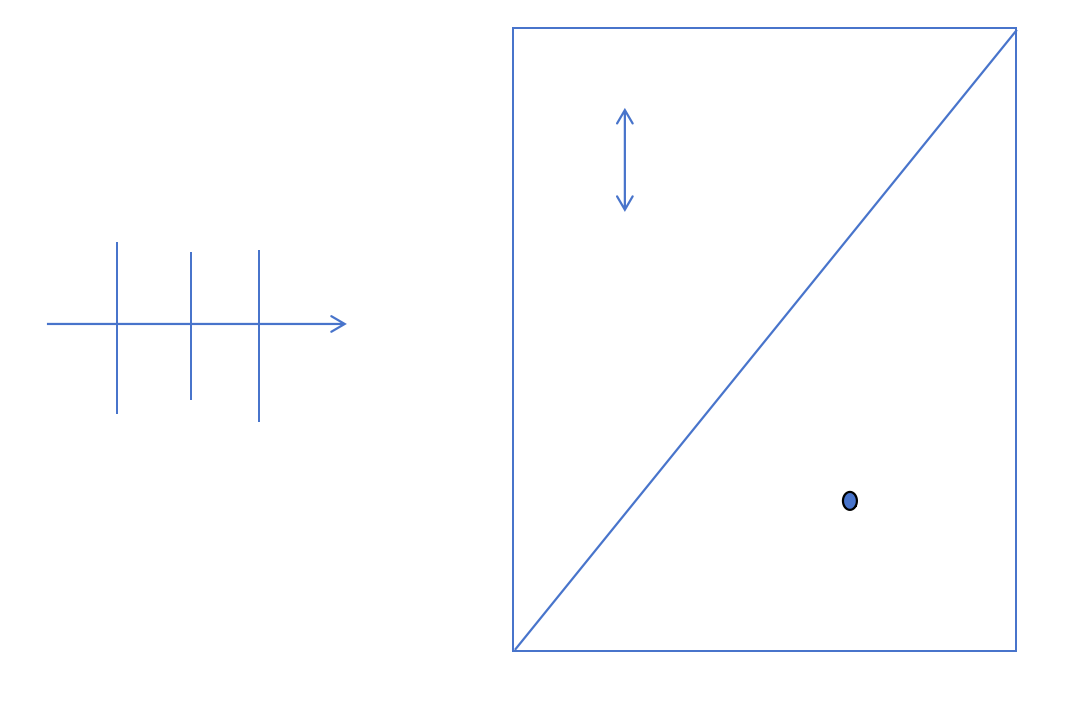
\includegraphics[width=0.7\linewidth]{07.png}
       
    \end{figure}
\end{enumerate}
\section*{三、简答题（32分）}
\begin{enumerate}
    \item 以知真空中一平面电磁波，其电场强度B可以表示为
    $B_x=0, B_y=66.7\times10^{-8}sin4\pi\times10^6(z-3\times10^8t), B_z=0$
    写出电场强渡E的表达式，此扰动的波长，速率和运动方向如何？
    \item 在双缝干涉实验中，两小孔的距离为1$mm$,屏到小孔的距离为1$m$,入射光波长为600$nm$和546$mm$,求:
    \begin{enumerate}
        \item 两光波分别形成条纹的间距
        \item 两组条纹的第十级亮纹之间的距离
    \end{enumerate}
    \item 纳光灯发射的黄光中包含两条相近的谱线称为纳双线$\lambda_1,\lambda_2$,平均波长589.3$nm$,利用纳黄光作为迈克尔逊干涉实验的光源，发现干涉场的可见度随平面镜的移动周期性变化，从条纹最清晰到最模糊总共变化490个条纹，求纳双线的波长差$\Delta\lambda$和他们的波长值。
    \item 导出单色光垂直入射光栅时，光谱线的角半宽度表达式，如果光栅宽度为10$cm$，每毫米内有500条缝，他产生的波长$\lambda=623nm$的单色光的一级谱线和二级谱线的角半宽度为多少？





\end{enumerate}

\end{document}